\section{Theorie}
\label{sec:theorie}

Vielfältige physikalische Prozesse sorgen dafür, dass in sämtlichen elektrischen Bauteilen ständig Schwankungen von Potentialen und somit Wechselspannungen auftreten. Diese Schwankungen resultieren aus statistischen Fluktuationen und sind daher nur sehr sehr klein. So entstehen zum Beispiel an Widerständen oder zwischen den Kathoden und Anoden von Röhren Wechselspannungen. Diese elektrischen Schwankungserscheinungen haben auf Präzisionsmessungen durchaus Auswirkungen und ihr Verständnis ist daher sehr nützlich. Analog zum Rauschen eines Lautsprechers durch statistische Fluktuationen der anliegenden Spannung wird dieses Phänomen auch Rauschen genannt.

Es sind verschiedene Arten von elektrischem Rauschen bekannt. Sie unterscheiden sich in ihrem Frequenzverhalten und spielen für verschiedene Bauteile unterschiedliche Rollen. Das \textbf{thermische Rauschen} erzeugt Spannungsschwankungen an ohmschen Widerständen. Bei Elektronenröhren werden durch die statistische Schwankung der Anzahl der austretenden Elektronen Schwankungen des zwischen der Anode und Kathode fließenden Stromes erzeugt. Hierbei handelt es sich um einen Effekt, der auch von der Geometrie des Bauteils abhängt. Er wird \textbf{Schrot-Effekt} genannt. Andere Fluktuationen können durch die zeitliche Änderung der Austrittsarbeit des Anodenmaterials entstehen. Dieser Prozess wird \textbf{Funkel-Effekt} genannt. Weil es sich bei all diesen Prozessen um statistisch auftretende Prozesse handelt, verschwindet der Mittelwert der Rauschspannung über große Dauern betrachtet.
%
\begin{equation}
  \bar{U}(t)=\lim_{\tau\rightarrow\infty}\int_0^\tau U(t)\upd t=0
\end{equation}
%
Daher wird in diesem Versuch der Mittelwert der quadrierten Rauschspannung untersucht. Dieser ist wie folgt definiert und insbesondere für große Zeitspannen unabhängig von diesen.
%
\begin{equation}
  \bar{U^2}(t) =\frac{1}{\tau}\int_0^\tau U^2(t) \upd t
\end{equation}
%
Diese Schwankungen werden daher auch \textit{stationäre Schwankungserscheinungen} genannt. Weil bei all diesen Prozessen fundamentale physikalische Prozesse verantwortlich sind, verknüpft die Messung die makroskopische Größe des Rauschspannungsquadrates mit physikalischen Naturkonstanten.

\subsection{Thermisches Rauschen und die Nyquist-Beziehung}
%
Wird die Spannung betrachtet, so stellt eine Doppelleitung der Länge $L$ bestehend aus zwei ohmschen Widerständen ein schwingfähiges System dar. Ein Schaltbild ist in Abbildung~\ref{fig:doppelleitung} dargestellt.
%
\begin{figure}
  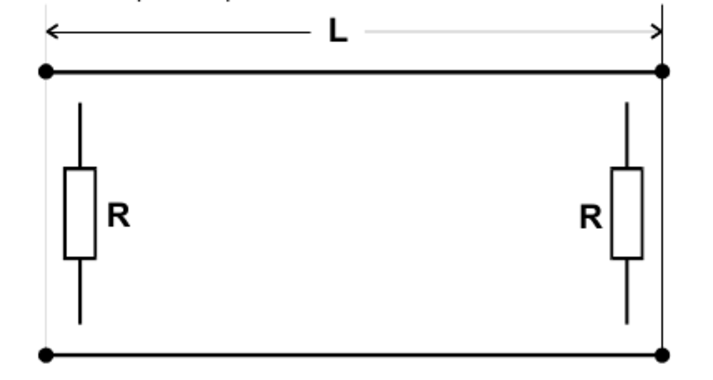
\includegraphics[width=0.8\textwidth]{figures/Doppelleitung.pdf}
  \caption{Schematisches Schaltbild einer Doppelleitung der Länge $L$ mit zwei ohmschen Widerständen \cite{V57}.}
  \label{fig:doppelleitung}
\end{figure}
%
Die Geometrie dieser Leitung legt dabei die möglichen Frequenzen der Schwingungen fest. Somit ist auch die Anzahl $\upD n$ der Eigenschwingungen in einem Frequenzintervall $\upD\nu$ festgelegt.
%
\begin{equation}
  \upD n=\frac{2\symup{L}}{v_\text{Ph}}\upD\nu
\end{equation}
%
Der Gleichverteilungssatz der statistischen Thermodynamik ordnet nun jeder Schwingung der Frequenz $\nu$ eine mittlere Energie zu:
%
\begin{equation}
  \upD n\bar{E}=\frac{\symup{h}\nu}{\exp{\frac{\symup{h}\nu}{\symup{k_\text{B}}T}}-1}\frac{2\symup{L}}{v_\text{Ph}}\upD\nu
\end{equation}
%
Für die Leistung $P$ pro Frequenzintervall $\upD\nu$ folgt daraus
%
\begin{equation}
  P=\frac{\symup{h}\nu}{\exp{\frac{\symup{h}\nu}{\symup{k_\text{B}}T}}-1}\upD\nu\; .
\end{equation}
%
Wird in dem Aufbau nun berücksichtigt, dass die Widerstände Energie aus der Schwingung absorbieren, indem sie diese in unzugängliche Wärmeenergie umwandeln, so findet nicht mehr unbedingt eine Schwingung statt. Eine stationäre Schwingung ist nur dann möglich, wenn die in Wärme umgewandelte Energie durch Rauschspannungen der Widerstände ausgeglichen wird. Die maximale Leistung, die durch das thermische Rauschen eines Widerstandes dabei zur Verfügung steht wird durch das gemittelte Rauschstromquadrat festgelegt. Sie wird erreicht, wenn der Wellenwiderstand $Z$ in der Leitung dem ohmschen Widerstand $R$ entspricht.
%
\begin{equation}
  \bar{N}_\text{max}=\frac{\bar{U^2}}{4R}=P
\end{equation}
%
Das mittlere Rauschspannungsquadrat ergibt sich daraus zu
%
\begin{equation}
  \bar{U^2}(\nu)=4RP=4R\frac{\symup{h}\nu}{\exp{\frac{\symup{h}\nu}{\symup{k_\text{B}}T}}-1}\upD\nu\\; .
\end{equation}
%
Durch Näherung der Exponentialfunktion folgt schließlich die \textsc{Nyquist}-Beziehung.
%
\begin{equation}
  \bar{U^2}=4\symup{k_\text{B}}T\cdot R\cdot\upD\nu
\end{equation}
%
Sie beschreibt ein weißes Rauschen, also ein Rauschen, welchges unabhängig von der Breite des Frequenzbandes ist.
